%--------------------------------------------------------------------------
\chapter{Testing laryngeal complexity in SLZ} \label{ch:testing_lc}
%--------------------------------------------------------------------------

%--------------------------------------------------------------------------
\section{Introduction}\label{sec:introduction_of_lc}
%--------------------------------------------------------------------------

This chapter investigates the role that laryngeal complexity plays in Santiago Laxopa Zapotec. Laryngeal complexity is used to describe the contrastive use of both tone and phonation in many languages, especially in the Oto-Manguean languages \citep{blankenshipTimeCourseBreathiness1997,blankenshipTimingNonmodalPhonation2002,silvermanLaryngealComplexityOtomanguean1997,silvermanPhasingRecoverability1997}. As mentioned in Chapter~\ref{ch:SLZ}, SLZ is a laryngeally complex language, because of its contrastive use of both tone and phonation. This means that SLZ can be used to test the predictions of laryngeal complexity, in regards to the phasing and recoverability of tone and phonation.

The goal of this chapter is to show that laryngeal complexity is present in SLZ as evidenced by the phasing of nonmodal phonation in several acoustic measures. This is done by looking at the acoustic properties of SLZ phonation using a combination of Strength of Excitation (SoE), Harmonic-to-Noise Ratio (HNR) < 1500 Hz and \textit{f}0 perturbations. It will be shown that there is a clear phasing between modal and nonmodal phonation in vowels that are described as breathy, checked, and rearticulated. 

These measures were selected based on the results of the MDS analysis in Chapter~\ref{ch:acousticlandscape} and the Random Forest analysis in Chapter~\ref{ch:revealing_trees}. Both the MDS and Random Forest analyses showed that SoE and HNR < 1500 Hz were the most important measures for distinguishing between the different phonation types. SoE has been used previously to show that there is clear phasing between modal and rearticulated vowels in San Sebastián del Monte Mixtec \citep{wellerInteractionsToneGlottalization2023,wellerLexicalToneVowel2023,wellerVoiceQualityTone2024}. 

HNR < 1500 Hz has not been used to date to show phasing between modal and nonmodal phonation. As a harmonics-to-noise ratio measure, HNR < 1500 Hz is a measure of the noise in the signal. This means that it can be used to determine if there is aperiodicity in the signal, which is one of the defining characteristics of nonmodal phonation \citep{ladefogedSoundsWorldsLanguages1996}. This means that HNR < 1500 Hz can be used to determine if there is a clear phasing between modal and nonmodal phonation in these vowels. 

Additionally, \textit{f}0 perturbation has been used previously to show that there is phasing between modal and nonmodal phonation in several Oto-Manguean languages \citep{garellekAcousticConsequencesPhonation2011,dicanioCoarticulationToneGlottal2012,keltererPhonationTypeContrasts2020}. 

The rest of this chapter will be organized as follows. First, I will provide a brief overview of laryngeal complexity and the phasing and recoverability of tone and phonation in Section~\ref{sec:what_is_lc}. In Section~\ref{sec:previous_analyses} I will discuss previous analyses of laryngeal complexity. In Section~\ref{sec:analysis_of_lc} I will discuss the methods used to analyze laryngeal complexity in SLZ. In Section~\ref{sec:results_of_lc} I will present the results of the analysis. Finally, in Section~\ref{sec:discussion_of_lc} I will discuss the implications of these results for our understanding of laryngeal complexity in SLZ.

%--------------------------------------------------------------------------
\section{What is Laryngeal Complexity?}\label{sec:what_is_lc}
%--------------------------------------------------------------------------

Laryngeal complexity is defined as the contrastive use of tone and phonation within the same syllablic nucleus \citep{blankenshipTimeCourseBreathiness1997,blankenshipTimingNonmodalPhonation2002,silvermanLaryngealComplexityOtomanguean1997,silvermanPhasingRecoverability1997}. This use of contrastive tone and phonation is one of the defining characteristics of the Oto-Manguean languages \citep{silvermanLaryngealComplexityOtomanguean1997}. However, it is not limited to just these languages. It has also been used to describe the behavior of tone or pitch in languages outside of the Oto-Manguean languages; such as the Tibeto-Burman languages of Mpi and Tamang \citep{silvermanLaryngealComplexityOtomanguean1997,silvermanPhasingRecoverability1997}, the Mayan language Yucatec Mayan \citep{frazierPhoneticsYucatecMaya2013}, and to describe the behavior of coarticulatory pitch and phonation in the Germanic language Danish \citep{frazierPhoneticsYucatecMaya2013,penaStodTimingDomain2022,penaProductionPerceptionStod2024}.

According to \citet{silvermanLaryngealComplexityOtomanguean1997,silvermanPhasingRecoverability1997}, even though tone and phonation are apparently allowed to co-occur in the same syllabic nucleus they are not allowed to be realized at the same time. \citeauthor{silvermanLaryngealComplexityOtomanguean1997} argues that this is because they are in competition with one another over the same articulatory gestures and perceptual resources. This means that tone and phonation must be realized in a temporally ordered fashion. This is what \citeauthor{silvermanLaryngealComplexityOtomanguean1997} refers to as phasing. Phasing is the idea that the two components of laryngeal complexity, tone and phonation, are temporally ordered with respect to one another. This means that one portion of the vowel is realized with modal phonation with the acoustic correlates of tone and the other portion of the vowel is realized with non-modal phonation with the acoustic correlates of said phonation. This phasing is also closely linked to the second main concept of laryngeal complexity, recoverability. Recoverability is the idea that the listener must be able to recover the underlying phonation and tone from the signal. These two concepts will be discussed in more detail in Section~\ref{sec:phasing_and_recoverability}.

%--------------------------------------------------------------------------
\subsection{Phasing and recoverability}\label{sec:phasing_and_recoverability}
%--------------------------------------------------------------------------

According to \citet{silvermanLaryngealComplexityOtomanguean1997,silvermanPhasingRecoverability1997}, one of the defining aspects of laryngeal complexity is the concept of phasing and recoverability. Under this idea, in laryngeally complex vowels the phonation and tone are phased with respect to one another in way that lends itself to a listener's ability to recover the underlying phonation and tone. In practical terms this means that laryngeally complex vowels are composed of two components: a modal voice portion of the vowel where tone is realized, and a non-modal voice portion of the vowel where phonation is realized. For the researcher that means that there are two distinct portions of the vowel that can be analyzed separately and that need to be analyzed temporally rather than spectrally \citep[237]{silvermanLaryngealComplexityOtomanguean1997}.

For example, in the Oto-Manguean language Jalapa Mazatec, breathiness or creakiness is realized only on the first portion of the vowel either as full laryngeal consonant or as a laryngeal feature on the vowel \citep[238]{silvermanLaryngealComplexityOtomanguean1997}. The second portion of the vowel is realized as a modal voice vowel with one of the three tones belonging to the tonemes of the language. This means that the breathiness or creakiness is phased with respect to the tone.

\citeauthor{silvermanLaryngealComplexityOtomanguean1997} argues that there are three principles that help explain why laryngeal complexity needs to be temporally ordered or phased: (i) sufficient acoustic distance, (ii) sufficient articulatory compatibility, and (iii) optimal auditory salience. 

%--------------------------------------------------------------------------
\subsubsection{Sufficient acoustic distance}\label{sec:sufficient_acoustic_distance}
%--------------------------------------------------------------------------

\citet{silvermanLaryngealComplexityOtomanguean1997} argues that sufficient acoustic distance is necessary for the recoverability of the phonation and tone. As Silverman explain, listeners do not rely on the fundamental frequency alone to perceive pitch. Instead, listeners use the harmonic spacing and the pulse period in the signal to perceive pitch \citep{ritsmaFrequenciesDominantPerception1967,remezIntonationSinusoidalSentences1993}. For modal phonation, this means that the harmonic spacing and pulse periods are present and encode a salient pitch value. However, during non-modal phonation, the harmonic spacing and pulse periods are often obscured or not present.

For breathy voice, this means that there is a general weakening 
of the harmonic structure which makes it difficult to recover the pitch by the listener \citep{silvermanPhasingRecoverability1997}. Creaky voice on the other had obscures the pulse periods due to its aperiodic and unstable glottal vibration \citep{ladefogedSoundsWorldsLanguages1996}. This is what was observed in Mazatec where the harmonic structure is gone and the pulses are indiscernible \citep{kirkQuantifyingAcousticProperties1993}. Additionally, the perception of pitch is rendered indiscernible when the pulse periods are varied by 10\% or more \citep{rosenbergPitchDiscriminationJittered1966}.

These observations lead \citet{silvermanLaryngealComplexityOtomanguean1997} to conclude that if a period glottal wave is either obscured (as with breathy voice) or not present (as with creaky voice), the acoustic signal cannot encode a salient pitch value. This means that the phonation and tone must be phased with respect to one another in order for the listener to recover the underlying phonation and tone. I will return to this point in Section~\ref{sec:discussion_of_lc}.

%--------------------------------------------------------------------------
\subsubsection{Sufficient articulatory compatibility}\label{sec:sufficient_articulatory_compatibility}
%--------------------------------------------------------------------------

Another important point for the \citeauthor{silvermanLaryngealComplexityOtomanguean1997}'s theory about laryngeal complexity has to deal with the articulatory compatibility of the phonation and tone. One of the guiding ideas behind this principle is that there is a principle of least effort in biological motor systems such as with speech production \citep{lindblomEconomySpeechGestures1983}. According to \citet{lindblomEconomySpeechGestures1983}, speech gestures can be thought of as distinct motor goals in our speech production system. These goals are achieved by the speaker through the coordination of the articulators with the least amount of effort. This means that that the gestures are coordinated in such a way that they are compatible with one another. This manifests itself either through sequencing or coarticulation of the gestures.

A good example of this comes from nasalization. In nasal contexts, the velum is lowered to allow air to pass through the nasal cavity, creating a nasal sound. This velum lowering gesture is compatible with the gestures needed in the oral cavity to produce different vowel qualities. This is what leads to the production of nasal vowels in languages like French or Portuguese. Additionally, this lowering also occurs in languages that do not have contrastive nasal vowels, such as English, where the velum is lowered in anticipation of a nasal consonant. This lowering of the velum is compatible with the gestures needed to produce the vowels in the oral cavity \citep[e.g.,][]{ohalaPhoneticExplanationsNasal1975,chenAcousticCorrelatesEnglish1997,stylerAcousticalPerceptualFeatures2015}.

According to \citeauthor{silvermanLaryngealComplexityOtomanguean1997}'s theory of laryngeal complexity, this idea of articulatory compatibility is also driving the need to phase phonation and tone. In the case of laryngeal complexity this is because it is assumed that both tone and phonation are produced by the larynx, more specifically the vocal folds and the glottis. This comes from early work on phonation and tone. For tone, \citet{ohalaProductionTone1978} showed that pitch was controlled primarily by the tensing or laxing of the vocal folds which changed the rate at which the vocal folds vibrate. For phonation, it was similarly shown that the amount the vocal folds where held open or closed determined the type of phonation that was produced \citep{ladefogedSoundsWorldsLanguages1996}. This aspect of phonation was shown in Figure~\ref{fig:phonation_types} and repeated here as Figure~\ref{fig:phonation_types_repeat}. 

\begin{figure}[h!]
    \centering
    \begin{tikzpicture}
        % Draw the line with arrows at both ends
        \draw[<->, line width=0.5mm] (0,0) -- (10,0);
        
        % Labels underneath the line
        \node[below] at (0,0) {[h]};
        \node[below] at (2,0) {Breathy};
        \node[below] at (5,0) {Modal};
        \node[below] at (8,0) {Creaky};
        \node[below] at (10,0) {[ʔ]};
        
        % Labels above the line
        \node[above] at (0,0) {Open Glottis};
        \node[above] at (10,0) {Closed Glottis};
    \end{tikzpicture}
    \caption{A diagram showing the relationship between breathy, modal, and creaky phonation types. Based on \citet{gordonPhonationTypesCrosslinguistic2001}.}
    \label{fig:phonation_types_repeat}
\end{figure}

For \citeauthor{silvermanLaryngealComplexityOtomanguean1997}'s \citeyear{silvermanLaryngealComplexityOtomanguean1997} theory of laryngeal complexity, the articulatory mechanisms for tone and phonation are exactly the same which leads to a need to phase the two in order to optimally make use of the same articulatory gestures. However, there is a growing body of literature that shows that tone and phonation is much more complex and is reliant on the entire larynx not just the vocal folds (e.g., \cite{eslingVoiceQualityLaryngeal2019}). This matter will be picked up again in Section~\ref{sec:discussion_of_lc}.

%--------------------------------------------------------------------------
\subsubsection{Optimal auditory salience}\label{sec:optimal_auditory_salience}
%--------------------------------------------------------------------------


%--------------------------------------------------------------------------
\subsection{Implicational hierarchy of laryngealization}\label{sec:implicational_hierarchy}
%--------------------------------------------------------------------------

Another aspect of \citeauthor{silvermanLaryngealComplexityOtomanguean1997}'s \citeyear{silvermanLaryngealComplexityOtomanguean1997} laryngeal complexity theory is that there is an implicational hierarchy in the phasing and ordering of phonation and tone. This hierarchy is based on how laryngealization appears in three Oto-Manguean languages. In this implicational hierarchy laryngealization can only appear in three ways: prevocalic, postvocalic, or interrupted. In the prevocalic case, the laryngealization appears before the vowel. In the postvocalic case, the laryngealization appears after the vowel. In the interrupted case, the laryngealization interrupts a vowel and appears in the middle.

According to \citet{silvermanLaryngealComplexityOtomanguean1997}, if a language has interrupted laryngealization, it must also have postvocalic laryngealization. If a language has postvocalic laryngealization, it must also have prevocalic laryngealization. In support of his claims \citet{silvermanLaryngealComplexityOtomanguean1997} provides data from three Oto-Manguean languages: Jalapa Mazatec, Comaltepec Chinantec, and Copala Trique. These languages are shown in Table~\ref{tab:implicational_hierarchy}.

\begin{table}[h!]
    \centering
    \caption{Implicational hierarchy of laryngeal complexity. The symbols h and ʔ represent laryngealization. The symbol V represents where the modal vowel is located in relation to the laryngealization.  Modified from \citet{silvermanLaryngealComplexityOtomanguean1997}.} 
    \label{tab:implicational_hierarchy}
    \begin{tabular}{lccc}
        \lsptoprule
        \textbf{Language} & \textbf{Prevocalic} & \textbf{Postvocalic} & \textbf{Interrupted} \\
        \hline 
        Jalapa Mazatec & hV˥, ʔV˥ & $-$ & $-$ \\
        Comaltepec Chinantec & hV˥, ʔV˥ & Vh˥, Vʔ˥ & $-$ \\
        Copala Trique & hV˥, ʔV˥ & Vh˥, Vʔ˥ & VhV˥, VʔV˥ \\
        \lspbottomrule
    \end{tabular}
\end{table}

For many descripitions of languages with laryngeal complexity, the implicational hierarchy seems to hold. This is certainly the case in the other Trique languages \citep{dicanioPhoneticsPhonologySan2008,dicanioItunyosoTrique2010,dicanioCoarticulationToneGlottal2012,dicanioPhoneticsFortisLenis2012,dicanioCueWeightPerception2014,dicanioGlottalTogglingItunyoso2020,elliottChicahuaxtlaTriqui2016,hollenbachPhonologyMorphologyTone1984}. However, as mentioned by \citet{frazierPhoneticsYucatecMaya2013}, it is not clear how accurate or robust this implicational hierarchy actually is. The reason for this is because it is not always clear if something is a laryngeal consonant or a laryngeal feature on the vowel. Indeed, \citet{silvermanLaryngealComplexityOtomanguean1997,silvermanPhasingRecoverability1997} treats laryngeal consonants and laryngeal features on vowels as the same thing. For example, in many of the Trique languages, the laryngealization is realized as a laryngeal consonant \citep{dicanioPhoneticsPhonologySan2008,dicanioItunyosoTrique2010,dicanioCoarticulationToneGlottal2012,dicanioPhoneticsFortisLenis2012,dicanioCueWeightPerception2014,dicanioGlottalTogglingItunyoso2020,elliottChicahuaxtlaTriqui2016,hollenbachPhonologyMorphologyTone1984}, but in Jalapa Mazatec, the laryngealization is realized as a laryngeal feature on the vowel \citep{kirkQuantifyingAcousticProperties1993,garellekAcousticConsequencesPhonation2011}. 

Another issue with the implicational hierarchy is that it is based on only three languages. This is a rather small sample size and doesn't capture the full range of variation in the Oto-Manguean languages. For example, in many Mixtec languages, laryngealization is understood to be a feature of the vowel rather than a consonant \citep[e.g.,][]{cortesSanSebastianMonte2023,eischensTonePhonationPhonologyPhonetics2022,gerfenPhonologyPhoneticsCoatzospan1999,gerfenProductionPerceptionLaryngealized2005}. Additionally, in many of this languages, the larngealization can appear either in the middle of the vowel, what \citet{silvermanLaryngealComplexityOtomanguean1997} calls interrupted, or at the end of the vowel \citep[e.g.,][]{cortesSanSebastianMonte2023,eischensTonePhonationPhonologyPhonetics2022}. This is directly in contrast to the implicational hierarchy which states that if a language has interrupted laryngealization, it must also have postvocalic laryngealization and prevocalic laryngealization.

Not only is the violation of the implicational hierarchy the case in Mixtecan languages, it is also the case in other branches of the Oto-Manguean languages. It is often the case that Zapotec languages only have interrupted and postvocalic vowels or just interrupted vowels (see \cite{ariza-garciaPhonationTypesTones2018} for a typology of phonation in Zapotec languages). For example, \citet{avelinoTopicsYalalagZapotec2004,avelinoAcousticElectroglottographicAnalyses2010} argues that Yalálag Zapotec only has interrupted laryngealization as a vowel feature and postvocalic laryngealization with a laryngeal consonant. However, there is no prevocalic laryngealization in the language. This is in direct contrast laryngeal complexity's implicational hierarchy. This is also true for laryngealization in Santa Ana del Valle Zapotec \citep{espositoSantaAnaValle2004,espositoAcousticElectroglottographicStudy2012}. This is also true for Santiago Laxopa Zapotec, where there is no prevocalic laryngealization despite having both interrupted and postvocalic laryngealization, see Chapter~\ref{ch:SLZ} for more detailed information.

%--------------------------------------------------------------------------
\section{Previous analyses of laryngeal complexity}\label{sec:previous_analyses}
%--------------------------------------------------------------------------

Previous analyses about laryngeal complexity fall into two categories: (i) descriptive studies and (ii) instrumental studies. In most descriptive studies, the focus has been on describing the patterns for tone and voice quality and how they interact with one another. For example, \citet{frazierPhoneticsYucatecMaya2013} describes the phonetic properties of tone and voice quality in Yucatec Mayan. In this study, \citeauthor{frazierPhoneticsYucatecMaya2013} describes how Yucatec Mayan is one of the few Mayan languages that has developed tonal contrasts. Additionally, it has a series of vowel that have high tone with glottalized that variably surface as either rearticulated vowels\footnote{This is very similar to rearticulated vowels in SLZ, where a vowel has a period of glottalization in the middle of the vowel that is often realized as a glottal stop. This is different from how \citet{bairdPhoneticPhonologicalRealizations2011} describes ``broken'' or ``rearticulated'' vowels in K'ichee' another Mayan language.} or as a vowel with creaky voice. \citeauthor{frazierPhoneticsYucatecMaya2013} notes that for most speakers these vowels show clear evidence of phasing between the tone and the voice quality. In these vowels the first portion of the vowel is always modal and produced with the high tone. The second portion of the vowel is produced with creaky voice which greatly obscures the pitch. 

Not only is this the case in Yucatec Mayan, but it is also the case in languages that primarily have a phonation contrast with tone/pitch as a secondary cue like Danish \citep{fischer-jorgensenPhoneticAnalysisStod1989,gronnumDanishStodLaryngealization2013,penaStodTimingDomain2022,penaProductionPerceptionStod2024}. In Danish, there is a phonation contrast that exists between modal voice and a type of creaky voice which is called stød. Research has shown that stød is also associated with a secondary cue of a heightened \textit{f}0 \citep{fischer-jorgensenPhoneticAnalysisStod1989,gronnumDanishStodLaryngealization2013}. \citet{penaStodTimingDomain2022,penaProductionPerceptionStod2024} showed that even though Danish is not traditionally classified as a laryngeally complex language it still shows evidence of phasing between the primary and secondary cues to stød, with the primary cue of phonation being produced in the second half of the syllablic rhyme and the secondary cue of pitch being produced in the first half of the syllablic rhyme.

In contrast to the descriptive studies, instrumental studies have focused on the acoustic properties of laryngeal complexity, primarily how laryngealization affects \textit{f}0 and the harmonic structure of the vowel. For example, \citet{garellekAcousticConsequencesPhonation2011} found that in Jalapa Mazatec, the laryngealization causes \textit{f}0 perturbation in the first portion of the vowel. \citeauthor{garellekAcousticConsequencesPhonation2011} conclude that this is evidence for the phasing between laryngealization and tone as predicted by \citeauthor{silvermanLaryngealComplexityOtomanguean1997}'s \citeyear{silvermanLaryngealComplexityOtomanguean1997} theory of laryngeal complexity. Additionally, this same phenomenon of \textit{f}0 perturbation has been shown to be the case with laryngealization in some varieties of Trique, again showing that there is phasing between modal and non-modal phonation \citep{dicanioCoarticulationToneGlottal2012}. For these previous studies the main piece of evidence for laryngeal complexity has been the perturbation of the \textit{f}0 signal in the portion of the vowel that is affected by the non-modal phonation.

In more recent studies, researchers have also looked at other measures besides \textit{f}0 to determine if there is phasing. For example \citet{wellerInteractionsToneGlottalization2023,wellerLexicalToneVowel2023,wellerVoiceQualityTone2024} have investigated laryngeal complexity in San Sebastián del Monte Mixtec using a combination of \textit{f}0 and Strength of Excitation (SoE), a measure that correlates to the strength of voicing, measures. They found that there is a clear phasing between modal and non-modal phonation in the rearticulated vowels of the language. 

However, these accounts only offer a limited window into the question of laryngeal complexity. Because there has been a focus on determining whether or not there are \textit{f}0 perturbations in the signal, these previous studies have missed the opportunity to look at the full range of acoustic properties. \citet{wellerInteractionsToneGlottalization2023,wellerLexicalToneVowel2023,wellerVoiceQualityTone2024} have done an excellent job by showing that by looking at SoE, in addition to \textit{f}0, we can get a better understanding of the phasing between tone and voice quality. However, there is still a need to look at other acoustic properties of the signal to get a full understanding of laryngeal complexity. 

The class of harmonic-to-noise ratio measures is one such class that promises to give this better understanding. Harmonic-to-noise ratio measures are a class of measures that look at the ratio of the harmonic energy to the noise energy in the signal. This class of measures has been particularly helpful in determining whether or not there is aperiodicity in the signal \citep{dekromCepstrumBasedTechniqueDetermining1993,ferrerriesgoWhatMakesCepstral2020,garellekPhoneticsVoice2019}. It is well understood that aperiodicity is one of the defining characteristics of non-modal phonation \citep{ladefogedSoundsWorldsLanguages1996}. This means that harmonic-to-noise ratio measures can be used to determine if there is aperiodicity in the signal and if there is a clear phasing between modal and non-modal phonation.

% The rest of this chapter will focus on analyzing SoE, a measure of the strength of voicing, and two harmonic-to-noise ratio measures, Harmonic-to-Noise Ratio (HNR) < 1500 Hz, which measures the noise in frequency band of 0 Hz to 1500 Hz, and Cepstral Peak Prominence (CPP), a measure of noise across the entire spectrum, in order to determine if there is a clear phasing between modal and non-modal phonation in SLZ using a generalized additive mixed model (GAMM) analysis \citep{hastieGeneralizedAdditiveModels1986,woodGeneralizedAdditiveModels2017,soskuthyGeneralisedAdditiveMixed2017,wielingAnalyzingDynamicPhonetic2018}.

%--------------------------------------------------------------------------
\section{Analysis of laryngeal complexity}\label{sec:analysis_of_lc}
%--------------------------------------------------------------------------



%--------------------------------------------------------------------------
\subsection{Methods} \label{sec:methods}
%--------------------------------------------------------------------------
%--------------------------------------------------------------------------
\subsubsection{Participants} \label{sec:participants}
%--------------------------------------------------------------------------
This study uses data collected from 10 native speakers of SLZ during the summer of 2022. Participants were recruited from the community of Santiago Laxopa, Oaxaca, Mexico. All participants were native speakers of SLZ. The participants were between 18 and 60 years old and consisted of five males and five females.

%--------------------------------------------------------------------------
\subsubsection{Recordings} \label{sec:recordings} 
%--------------------------------------------------------------------------
Participants were asked to perform a word list elicitation task consisting of 72 words. These words were selected to elicit the entire range of types of voice quality in SLZ, including modal voice, the two kinds of creaky (i.e., checked and rearticulated), and breathy voice. The words were selected based on previous research conducted as part of the Zapotec Language Project at the University of California, Santa Cruz \citep{ZapotecLanguageProject}. 
Because participants were not literate in SLZ, the word list was prompted for them by asking them ``How do you say [word in Spanish]?" by myself and another researcher in Zapotec. Participants were asked to respond with the desired word in the carrier phrase \textit{Shnia' X chonhe lhas} [ʃnːiaˀ X tʃone ɾas] ``I say X three times.'' which was repeated three times. These utterances were recorded in a quiet environment using a Zoom H4n handheld digital recorder. The recordings were saved as 16-bit WAV files with a sampling rate of 44.1 kHz.

%--------------------------------------------------------------------------
\subsubsection{Acoustic measuring} \label{sec:acoustics}
%--------------------------------------------------------------------------

% The resulting audio files were then processed in Praat to isolate the vowel portion of each word. The onset of the vowel was set to the second glottal pulse after the onset, and the offset of the vowel was set to the last glottal pulse before the decrease in amplitude at the end of the vowel \citep{garellekAcousticDiscriminabilityComplex2020}. The vowel was then extracted and saved as a separate file for analysis.

% These vowels were fed into VoiceSauce \citep{shueVoiceSauceProgramVoice2011} to generate the acoustic measures for the studies discussed in this dissertation. Because many acoustic measures are based on the fundamental frequency, this measure was calculated using the STRAIGHT algorithm from \citep{kawaharaInstantaneousfrequencybasedPitchExtraction1998} to estimate the fundamental frequency in millisecond (ms) intervals. Once the fundamental frequency is calculated, VoiceSauce then uses an optimization function to locate the harmonics of the spectrum, finding their amplitudes.

% VoiceSauce then uses the Snack Sound toolkit \citep{sjolanderSnackSoundToolkit2004} to find the frequencies and bandwidths of the first four formants, also at millisecond intervals. The amplitudes of the harmonics closest to these formant frequencies are located and treated as the amplitudes of the formants. These formant frequencies and bandwidths are used to correct the harmonic amplitudes for the filtering effects of the vocal tract, using \citeauthor{iseliAgeSexVowel2007}'s \citeyear{iseliAgeSexVowel2007} extension of the method employed by \citet{hansonGlottalCharacteristicsFemale1997}. Each vowel was measured across ten equal time intervals, resulting in 22890 data points in total. These measures were then z-scored by speaker to reduce the variation between speakers and provide a way to compare the different measures directly on similar scales.

% %--------------------------------------------------------------------------
% \subsubsection{Data processing} \label{sec:data_processing}
% %--------------------------------------------------------------------------
% Data points with an absolute z-score value greater than three were considered outliers and excluded from the analysis. The Mahalanobis distance was calculated in the F1-F2 panel within each vowel category. Each data point with a Mahalanobis distance greater than six was considered an outlier and excluded from the analysis. Using the Mahalanobis distance allows us to compare the data points to the mean of the F1-F2 panel for each vowel category. The larger the Mahalanobis distance is the more deviant the data point is from the mean which in turn means that the data point was improperly tracked. This is comparable to what was done in \citet{seyfarthPlosiveVoicingAcoustics2018,chaiCheckedSyllablesChecked2022,garellekPhoneticsWhiteHmong2023}.

% Energy was excluded if it had a zero value and then log-transformed to normalize its right-skewed distribution. Afterward, the resulting log-transformed Energy was z-scored, and any data point with a z-score greater than three was excluded. This outlier removal resulted in 1918 data points being removed. 

% All data points were then z-scored by speaker to reduce the variation between speakers and provide a way to compare the different measures directly on the same scale.

% Residual H1* for the remaining data points following \citet{chaiH1H2AcousticMeasure2022}. First, a linear mixed effects model was generated with the z-scored H1* as the response variable and the z-scored energy as the fixed effect. The uncorrelated interaction of the z-scored energy by speaker was treated as random. The energy factor resulting from this linear mixed-effects model was extracted. Finally, the z-scored H1* had the product of the z-scored energy and energy factor subtracted from it to produce the residual H1* measure.

% As was mentioned in Chapter~\ref{ch:residual_h1}, the distribution of tone and phonation was not equal across all combinations of the two. This means that in the dataset certain combinations of tone and phonation were overrepresented. As seen in Table~\ref{tab:distribution}, which is repeated here as Table~\ref{tab:distribution_repeat}, the distribution of tone and phonation is not equal across all combinations. 


% % \begin{table}[!h]
% %     \centering
% %     \caption{Distribution of the number of syllables containing the combination of tone and voice quality in the wordlist.}
% %     \label{tab:distribution_repeat}
% %       \begin{tabular}{llllll}
% %       \lsptoprule
% %       & High & Mid & Low & Rising & Falling\\
% %       \hline
% %       Modal & 14 & 9 & 15 & 2 & 10 \\
% %       Breathy & $-$ & $-$ & 11 & $-$ & 2 \\
% %       Checked & 1 & $-$ & 9 & $-$ & \\
% %       Rearticulated & 1 & $-$ & 4 & $-$ & 4 \\
% %       \lspbottomrule
% %       \end{tabular}
% % \end{table}

% % Modal voice was the only phonation that occurred across all possible tones and Low tone was the only tone that occurred across all possible phonations. This means that the dataset is not balanced and that there are more data points for certain combinations of tone and phonation than others. This is a problem because it can lead to biased results in the analysis for laryngeal complexity. To correct for this, only the phonations that occurred in low tone were used for the laryngeal complexity analysis. By limiting the analysis to only low tone, we ensure that the dataset is accurately capturing the effects of the interaction of phonation on a specific tone. Additionally, this will allow us to ignore the potential confound of how creaky voice is not uniformly produced when it appears with different tones \citep{keatingAcousticPropertiesDifferent2015}.

% %--------------------------------------------------------------------------
% \subsubsection{Statistical analysis} \label{sec:statistical_analysis}
% %--------------------------------------------------------------------------

% The data were analyzed using a generalized additive mixed model (GAMM) \citep{hastieGeneralizedAdditiveModels1986,woodGeneralizedAdditiveModels2017,soskuthyGeneralisedAdditiveMixed2017,wielingAnalyzingDynamicPhonetic2018}. The GAMM was fit using the \texttt{mgcv} package in R \citep{woodGeneralizedAdditiveModels2017}.


% %--------------------------------------------------------------------------
% \section{Results}\label{sec:results_of_lc}
% %--------------------------------------------------------------------------

% \begin{figure}[h!]
%     \centering
%     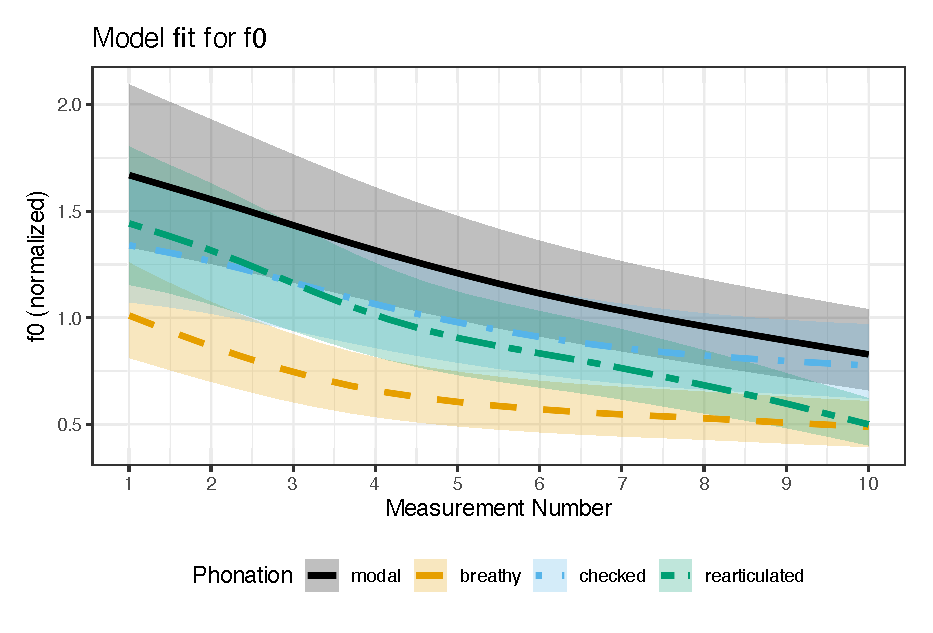
\includegraphics[]{images/LCH_GAMMs/f0_model_fit.eps}
%     \caption{Model fit for \textit{f}0.}
%     \label{fig:f0_model_fit}
% \end{figure}

% \begin{figure}[h!]
%     \centering
%     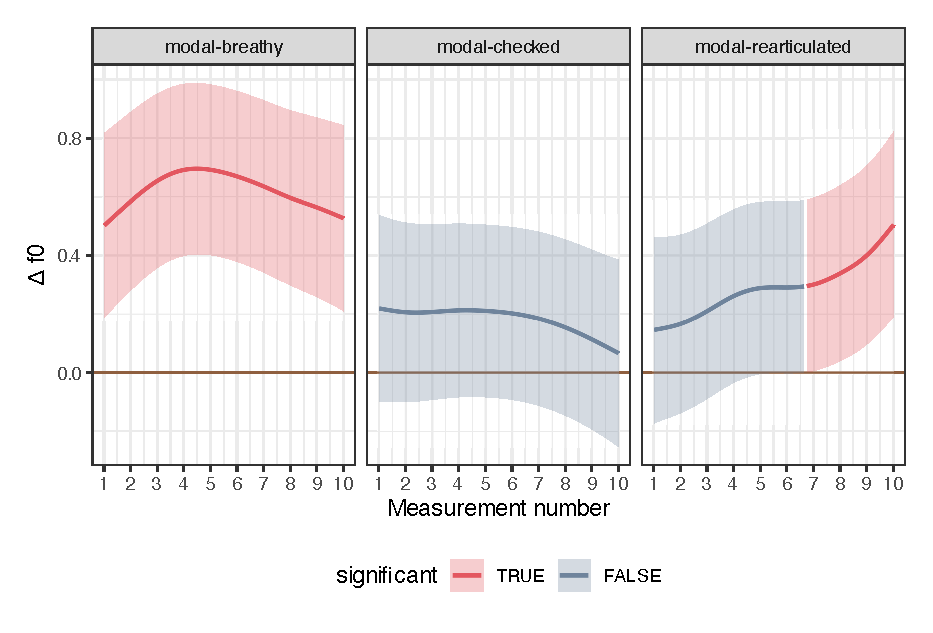
\includegraphics[]{images/LCH_GAMMs/f0_model_diff.eps}
%     \caption{Plot of the difference between modal and each of the non-modal phonation types.}
%     \label{fig:f0_model_diff}
% \end{figure}

% \begin{figure}[h!]
%     \centering
%     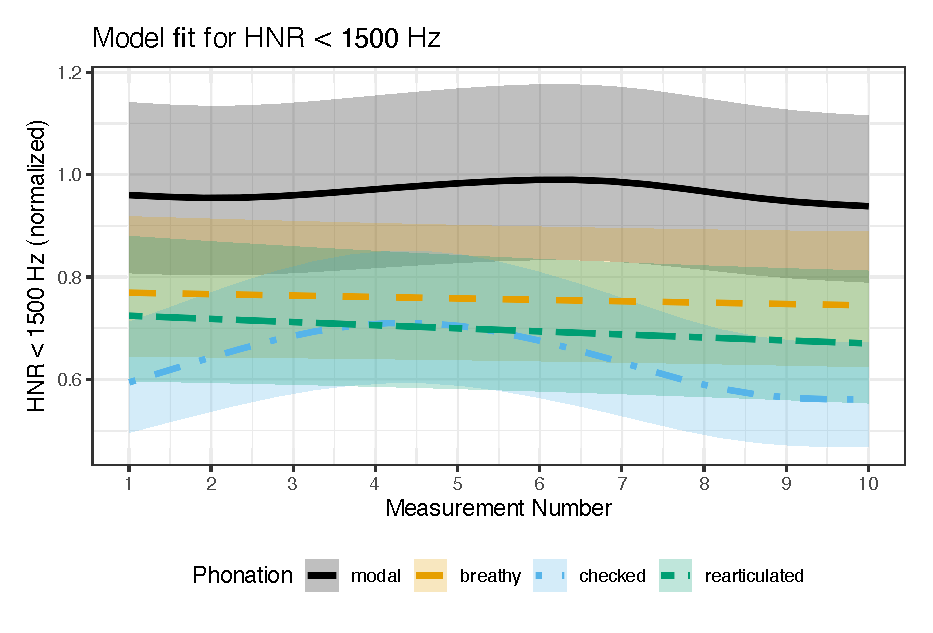
\includegraphics[]{images/LCH_GAMMs/hnr15_model_fit.eps}
%     \caption{Model fit for HNR.}
%     \label{fig:hnr_model_fit}
% \end{figure}    
% \begin{figure}[h!]
%     \centering
%     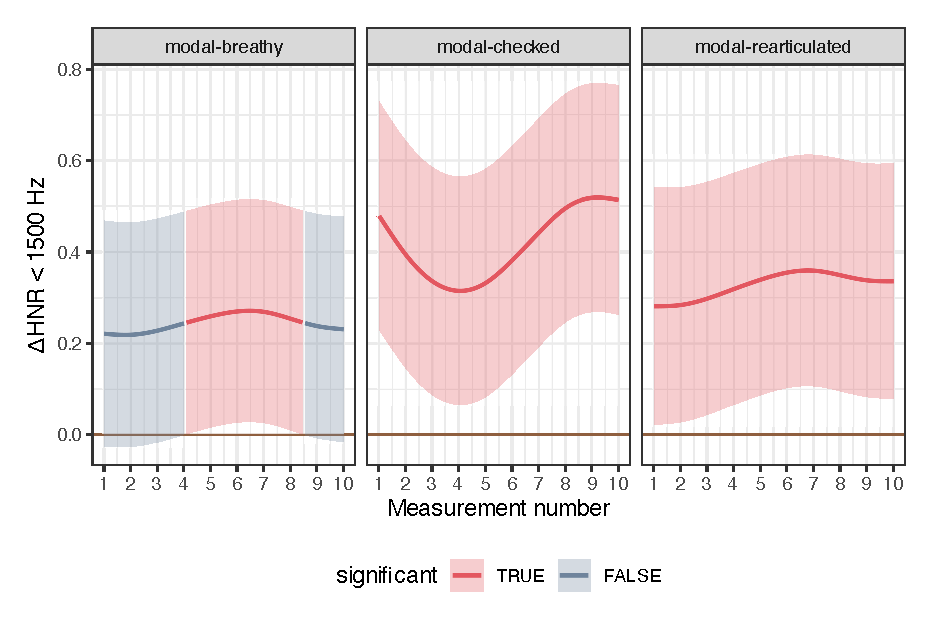
\includegraphics[]{images/LCH_GAMMs/hnr15_model_diff.eps}
%     \caption{Plot of the difference between modal and each of the non-modal phonation types.}
%     \label{fig:hnr_model_diff}
% \end{figure}

% \begin{figure}[h!]
%     \centering
%     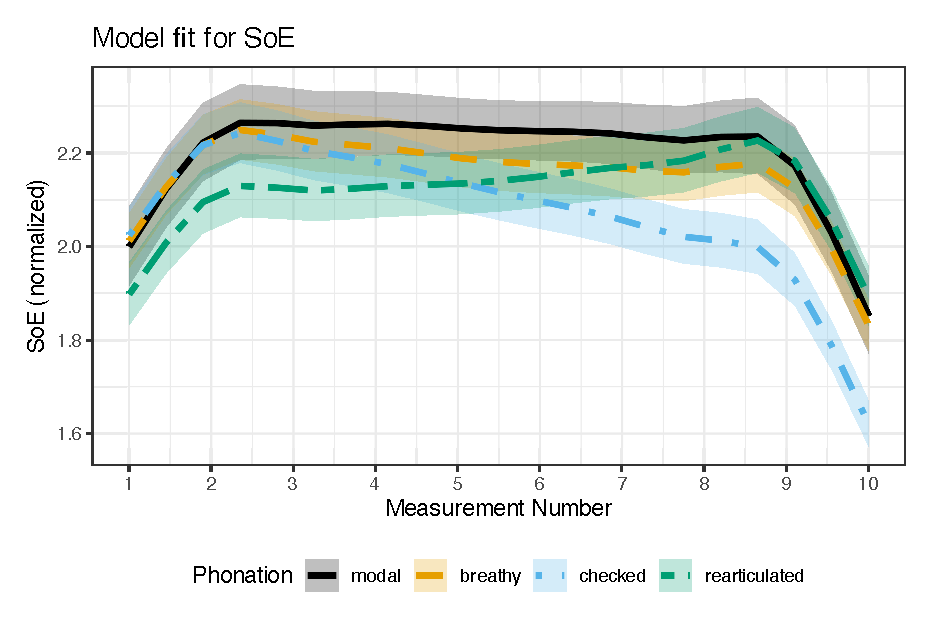
\includegraphics[]{images/LCH_GAMMs/soe_model_fit.eps}
%     \caption{Model fit for SoE.}
%     \label{fig:soe_model_fit}
% \end{figure}

% \begin{figure}[h!]
%     \centering
%     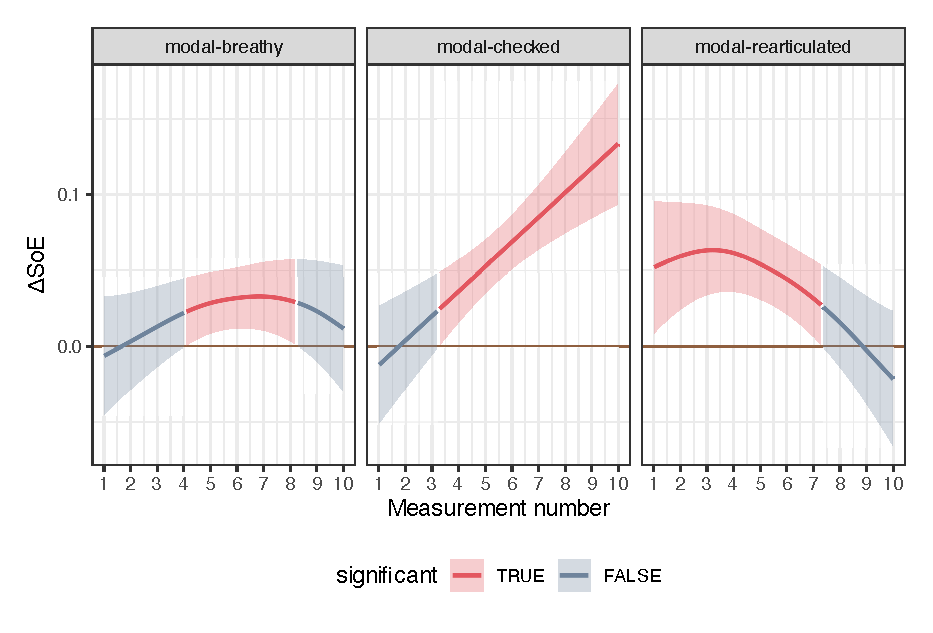
\includegraphics[]{images/LCH_GAMMs/soe_model_diff.eps}
%     \caption{Plot of the difference between modal and each of the non-modal phonation types.}
%     \label{fig:soe_model_diff}
% \end{figure}


% %--------------------------------------------------------------------------
% \section{Discussion}\label{sec:discussion_of_lc}
% %--------------------------------------------------------------------------

% \citet{humbertConsonantTypesVowel1978} 


% %--------------------------------------------------------------------------
% \section{Conclusion}\label{sec:conclusion_of_lc}
% %--------------------------------------------------------------------------
